\chapter{Σχεδίαση και Ανάλυση}

\section{Απαιτήσεις Συστήματος}




\subsection{Λειτουργικές απαιτήσεις}

\begin{itemize}
	\item Η δυνατότητα παροχής στον χρήστη ενός Γραφικού Περιβάλλοντος, μέσω του οποίου μπορεί να δημιουργεί αντικείμενα που θα χρησιμεύσουν ως βασικά στοιχεία για τις επόμενες λειτουργίες.
    \item Η δημιουργία λειτουργίας για τη δυνατότητα επίβλεψης της κατάστασης επιλεγόμενης διεπαφής.
    \item Η δημιουργία λειτουργίας για τη δυνατότητα επίβλεψης στατιστικών για επιλεγόμενη δικτυακή συσκευή.
    \item Η δημιουργία λειτουργίας για τη δυνατότητα επίβλεψης στατιστικών επιλεγόμενης διεπαφής.
    \item Η δημιουργία λειτουργίας για τη δυνατότητα συλλογής ως \en{backup} τρέχοντος \en{configuration}.
    \item Η δημιουργία λειτουργίας για τη δυνατότητα αλλαγής \en{IP} διεύθυνσης επιλεγόμενης δικτυακής εφαρμογής.
\end{itemize}

\subsection{Τοπικό περιβάλλον ανάπτυξης}

Το λογισμικό πάνω στο οποίο δοκιμάστηκε η εφαρμογή είναι \en{Linux}, \en{Ubuntu 22.04.2 LTS} η οποία εικονοποιήθηκε πάνω σε λειτουργκό \en{Windows} ως \en{WSL2}. 
Το \en{Windows Subsystem for Linux version 2} είναι μια τεχνολογία της \en{Microsoft} που επιτρέπει στους χρήστες \en{Windows} να τρέχουν \en{Linux} 
περιβάλλοντα απευθείας στο λειτουργικό σύστημα \en{Windows}, χωρίς την ανάγκη για εξομοιωτές ή εικονικές μηχανές. 
Είναι η δεύτερη έκδοση του \en{Windows Subsystem for Linux} και αποτελεί σημαντική βελτίωση σε σχέση με την πρώτη έκδοση \en{WSL1}. Το \en{WSL} 2 χρησιμοποιεί την τεχνολογία εικονικοποίησης (\en{virtualization}) για να 
τρέχει έναν πραγματικό πυρήνα \en{Linux} μέσα σε μια ελαφριά εικονική μηχανή βοηθητικών λειτουργιών (\en{utility VM}). Αυτό επιτρέπει στο \en{WSL} 2 να προσφέρει 
καλύτερη απόδοση, πλήρη συμβατότητα με τις λειτουργίες \en{Linux} και πρόσβαση σε εργαλεία όπως το \en{Docker}.

\section{Η επανάσταση στο \en{web development}}

Στην αρχή, οι εφαρμογές ιστού δεν ήταν τίποτα περισσότερο από ένα σύνολο αρχείων \en{HTML, CSS} και
\en{javascript} που ήταν συνδεδεμένα μεταξύ τους. Ένας καλός προγραμματιστής ήταν σε θέση να φτιάξει σπουδαίες εφαρμογές ιστού αν αυτός/αυτή
είχε αρκετές δεξιότητες/γνώσεις.

Στην εποχή μας, εμφανίστηκαν τα \en{frameworks} και λαμβάνοντας υπόψη ότι ουσιαστικά δεν βελτιώνουν αυτό που τελικά βλέπει ο χρήστης και τις
αλληλεπιδράσεις του με το \en{frontend}, τότε
θα μπορούσε κανείς να αναρωτηθεί γιατί χρησιμοποιούνται ευρέως στις μέρες μας.
Παρόμοιες δουλειές με την παρούσα εργασία υπάρχουν και σε άλλες διπλωματικές εργασίες καθώς και σε μη διπλωματικές εργασίες. Μηχανικοί από όλο τον κόσμο
ασχολούνται με την αυτοματοποίηση συστημάτων και τη δημιουργία κώδικα που να αυτοματοποιεί συσκευές/συστήματα. 

Με βάση άλλες τέτοιες προσπάθειες που έχουν γίνει στο παρελθόν εμείς συλλέξαμε την εως τώρα βιβλιογραφία
και προσπαθήσαμε να φτιάξουμε μία τέτοια εφαρμογή η οποία όμως να βασίζεται στα τωρινά δεδομένα και να 
ενσωματσώσουμε τις τελευταίες τεχνολογίες αιχμής όπως την \en{Cloud Native} αρχιτεκτονική. Στη συνέχεια γίνεται προσπάθεια να δωθεί εκτενής
ανάλυση στο πως λειτουργεί η εφαρμογή καθώς και στην αλληλλεπίδρασή της με τα συνεργαζόμενα συστήματα. 


\section{Αρχιτεκτονική της εφαρμογής}
 
\subsection{Μοντέλο \en{MVC} (\en{Model-View-Controller})}

Το μοτίβο \en{MVC} είναι ένα αρχιτεκτονικό μοτίβο ανάπτυξης λογισμικού που διαχωρίζει την παρουσίαση δεδομένων από τη λογική διαχείρισης των αλληλεπιδράσεων του 
χρήστη. Υπάρχει ως ιδέα εδώ και καιρό και έχει δει εκθετική αύξηση στη χρήση του από την εισαγωγή του. 
Επίσης, έχει χαρακτηριστεί ως ένας από τους καλύτερους τρόπους για τη δημιουργία εφαρμογών πελάτη-διακομιστή όπου ο χρήστης αντιλαμβάνεται ώς γραφικό περιβάλλον. 'Ολα τα κορυφαία \en{frameworks} 
για το \en{web} είναι βασισμένα στο \en{MVC}. 

Παρόλο που το \en{Django} ακολουθεί το μοτίβο \en{MVC}, προτιμά να χρησιμοποιεί τη δική του λογική στην υλοποίηση. Το \en{framework} αναλαμβάνει το \en{Controller} 
μέρος του \en{MVC} και αφήνει τα περισσότερα από τα "καλά" να γίνονται στο \en{Model-Template-View (MTV)}.

Αυτός είναι ο λόγος που το \en{Django} συχνά αναφέρεται ως \en{MTV framework}.


\section{\en{Django MTV}}
\begin{itemize}
    \item \en{Model:} Αντιπροσωπεύει τα δεδομένα και τη διαχείρισή τους.  
    \item \en{Template:} Εστιάζει στο τι βλέπει ο χρήστης 
    \item \en{View} Συνδέει το \en{Model} και το \en{Template}, διαχειριζόμενο τη λογική
\end{itemize}

Με άλλα λόγια, το \en{Django} κρατά την πολυπλοκότητα μακριά από τον προγραμματιστή, καθιστώντας την εμπειρία πιο απλή και παραγωγική.

\subsection{Διαγραμματική απεικόνιση της εφαρμογής}

\textbf{\en{Model}(Μοντέλο):}
Το \en{Device} είναι το κύριο μοντέλο που χρησιμοποιείται εδώ. Αναπαριστά τις δικτυακές συσκευές (π.χ. δρομολογητές, \en{switches}) και τις σχετικές πληροφορίες τους:

Πεδία όπως: \en{host}, \en{username}, \en{password}, \en{platform}, και \en{secret}.
Το μοντέλο αυτό συνδέεται με τη βάση δεδομένων και παρέχει \en{API} για \en{CRUD} λειτουργίες (\en{Create}, \en{Read}, \en{Update}, \en{Delete}). Το μοντέλο αυτό είναι η βάση δεδομένων μας.

\textbf{\en{Template} (Πρότυπο):}

Τα αρχεία \en{.html} είναι τα πρότυπα που χρησιμοποιούνται για την παρουσίαση δεδομένων. 

Προβολή λίστας συσκευών.
Παρουσίαση στατιστικών.
Εμφάνιση ρυθμίσεων διαμόρφωσης ή αποτελεσμάτων εκτέλεσης εντολών.
Χρησιμοποιούν τη γλώσσα \en{Django Template} για δυναμικό περιεχόμενο (π.χ., λίστες συσκευών, στατιστικά).

\textbf{\en{View} (Προβολή):}
Οι \en{views} είναι οι \en{Python} συναρτήσεις που:

Παίρνουν αιτήματα από τον χρήστη.
Επικοινωνούν με το μοντέλο για δεδομένα.
Επιστρέφουν απαντήσεις με τη μορφή \en{HTML}.

Στην εικόνα παρακάτω παρουσιάζεται διάγραμμα απεικόνισης της βασικής αρχιτεκτονικής της εφαρμογής.

\begin{figure}[h]
	\centering
	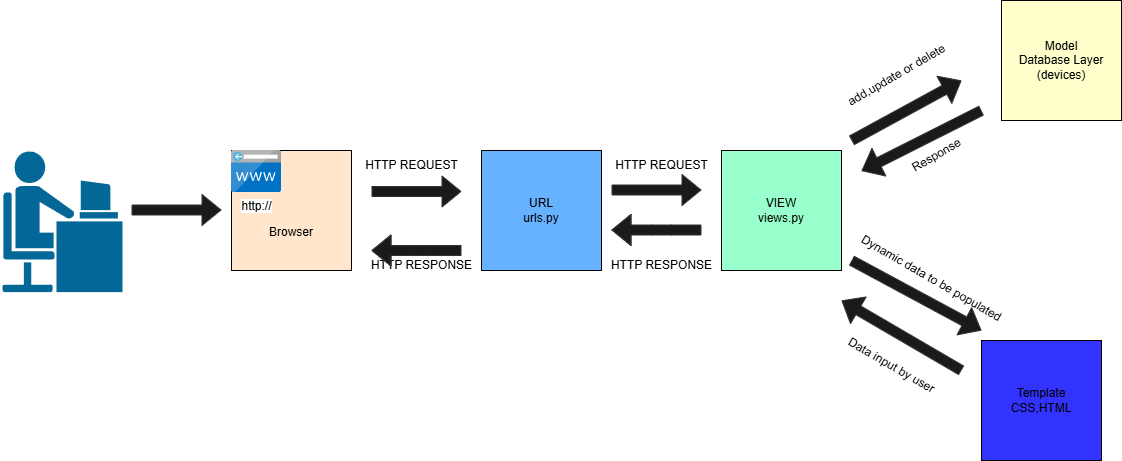
\includegraphics[width=0.7\textwidth]{graphics/MTV.drawio.png}
	\caption{\en{MTV}}
\end{figure}



\section{Εικονικό Περιβάλλον Δικτύου \en{GNS3 –Testbed}}



\subsection{Σχεδίαση Τοπολογίας Δικτύου}

Η λογική την οποία χρησιμοποιήσαμε για τη δημιουργία του \en{Testbed} 
είναι ότι οι συσκευές οι οποίες τρέχουν πάνω στο \en{GNS3 VM} θα μπορέσουν
να αλληλεπιδράσουν με το τοπικό \en{WSL2} περιβάλλον. Προκειμένου να επιτευχθεί αυτός ό στόχος
ακολουθήθηκαν βήματα. Το πρώτο βήμα είναι η εγκατάσταση βασικών προγραμμάτων τα οποία έχουν παρουσιαστεί στο Θεωρητικό υπόβαθρο.

Σε \en{High Level overview} η εφαρμογή ακολουθεί την παρακάτω τοπολογία:

\FloatBarrier

\begin{figure}[htb]
	\centering
	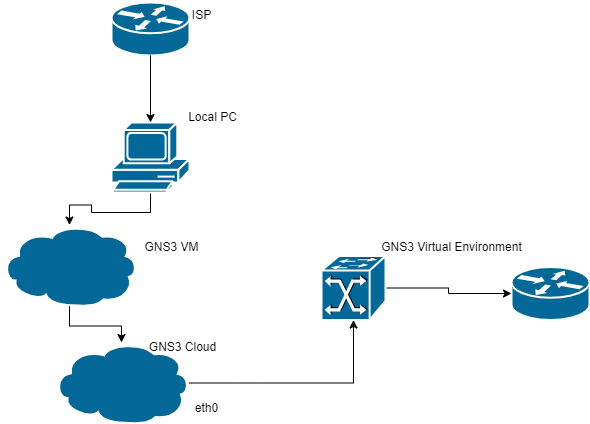
\includegraphics[width=0.7\textwidth]{graphics/diagram.drawio.png}
	\caption{\en{Local PC-GNS3VM-CISCO IOS Connection Architecture} }
\end{figure}


\subsection{Προσομοίωση Συσκευών \en{Cisco}}

Προκειμένου να προσομειώσουμε συσκευές της \en{Cisco} το πρώτο βήμα είναι να κατεβάσουμε συγκεκριμένο \en{appliance} απο το \en{GNS3 marketplace}.
Αφού το κατεβάσουμε το εισάγουμε στο \en{GNS3} με τον εξής τρόπο: (εικόνα 5.3)

\FloatBarrier

\begin{figure}[htb]
	\centering
	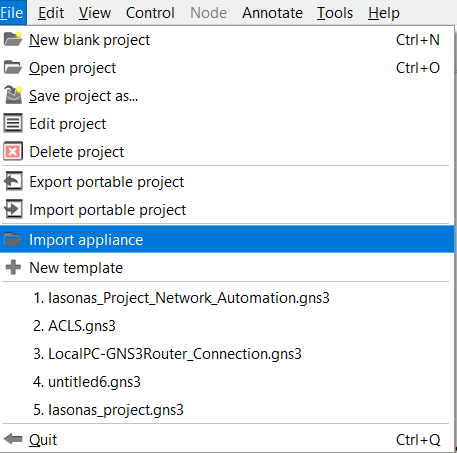
\includegraphics[width=0.7\textwidth]{graphics/import_appliance.png}
	\caption{\en{Import appliance} }
\end{figure}

Ακολούθως πατάμε \en{Install appliance on the GNS3 VM} και ματσάροντας το \en{filename} του \en{appliance} με το \en{image} που έχουμε μας επιτρέπει να εισάγουμε τη συσκευή.

Για να δούμε το \en{filename} στο \en{appliance} ανοίγουμε το αρχείο με έναν \en{editor} και αλλάζουμε το \en{filename} αντίστοιχα οπως στην  εικόνα 5.4.

\FloatBarrier

\begin{figure}[htb]
	\centering
	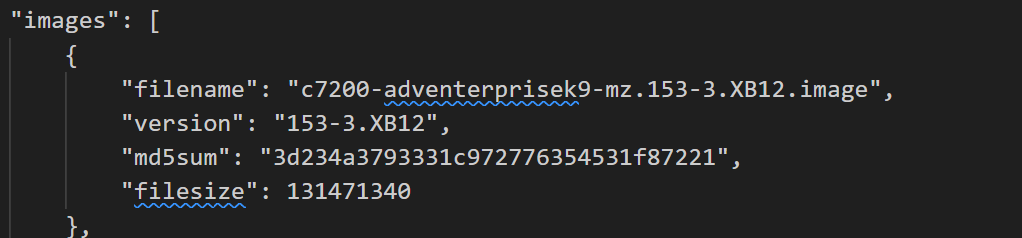
\includegraphics[width=0.7\textwidth]{graphics/appliance_filename.png}
	\caption{\en{filename configuration} }
\end{figure}

\FloatBarrier

Μετά το τέλος της διαδικασίας η συσκευή θα έχει προστεθεί και μπορούμε να την δούμε στην επιλογή \en{Browse all devices}

